\section{Discussion}
% refer lectures! 
% talk about improvements
%% write something under this title. Titles should not have no content underneath
\subsection{Using Theory in Practice}
%how you applied knowledge from lecture
When we design our state machine, we tend to add a lot more states which are similar to some other state in our satte machine. This was not a efficient way to design a state machine. So we tried to use a hierarchy structure to make our state machine reusable and more logical. From lecture 11, we learn to build a hierarchical finite state machine with historical transition. By this structure, our Kobuki can perform obstacle avoidance with in a run state, and can also perform a hill climb in a drive state. This structure improves the simplicity and readability of our state machine. %insert lecture 11 as a citation?
% using variables, preemption? maybe?... using LPF to treat sensitivity? L 3/4
\\
\colorbox{yellow}{Probably just try to finish filling page 17}

\clearpage
\subsection{Project Achievements}
% a bunch of stuff about what we did great and awesome and what should inspire other kids to do more of this
\vspace{-0.2cm} A summary of the achieved outcomes in testing/simulation and in the final obstacle course in line with the project requirements (see Section \ref{sec:requirements}) is shown in Table \ref{tab:outcomes}.
\begin{table}[H]
\centering
\begin{tabularx}{\textwidth}{|X|X|X|}
    \hline
    \begin{center}
        \textbf{Expected Outcomes - Requirements} (see Section \ref{sec:requirements})
    \end{center} & 
    \begin{center}
        \textbf{Simulation \& Testing Outcomes} (see Section \ref{sec:testing})
    \end{center} & 
    \begin{center}
        \textbf{Final Run Outcome} \hspace{1cm} (see Section \ref{sec:validation})
    \end{center}\\
    \hline
    \underline{Play/Pause:}
    Kobuki does not run until B0 is pressed.
    When running, Kobuki will be paused when B0 is pressed.
    After a paused state, when B0 is pressed again the Kobuki will resume from the state that it was paused.
    & All requirements were met in testing state outputs can be seen in Appendix \ref{app:play_pause_states}. CyberSim did not offer direct button control for B0 to simulate the play/pause function. 
    & Kobuki did not run until B0 is pressed at the starting line. When B0 was pressed it started the obstacle course. The run was terminated when B0 was pressed to pause the robot.\\
    \hline
    \underline{Obstacle Avoidance:}
    The Kobuki should avoid obstacles (cliffs, wheel hazards and objects) whilst driving.
    After encountering obstacles the Kobuki must reorient and resume driving in ground orientation.
    & Obstacle avoidance was observed in both simulation and Kobuki testing. The algorithm always made sure to \textit{Reverse}, \textit{TurnAway}, \textit{DriveAvoid}, \textit{TurnBack} and \textit{Drive}. Wheel hazards were not observed in simulation. On the Kobuki wheels were only a hazard when the speed was greater than 200mm/s. 
    & The Kobuki successfully avoided three obstacles but only managed to reorient back to ground orientation and drive on with the first two obstacles.
    \\
    \hline
    \underline{Hill Climb:}
    The Kobuki must be able to climb a hill, drive through a plateau, and descend to ground before stopping within 40cm from reaching ground.
    Whilst on an incline the Kobuki must reorient to drive in an orthogonal direction to the slope.
    The Kobuki must avoid cliffs on the incline.
    & All requirements were met in Kobuki testing with the final implemented hill climb algorithm. The state outputs can be seen in Appendix \ref{app:hill_states} going through \textit{Drive}, \textit{Ascending}, \textit{Top}, \textit{Descending} and \textit{End}, as well as, obstacle avoidance states \textit{Reverse}, \textit{TurnAway}, \textit{DriveAvoid}, and \textit{TurnBack}.
    & The Kobuki did not reach the hill climb section of the course and therefore did not get to generate hill climb outcomes.
    \\
    \hline
    \underline{Performance:}
    The Kobuki does not rotate more than $180^\circ$.
    Chattering and erratic movements should not be exhibited.
    Abnormal termination is not to occur.
    The Kobuki is not allowed to repeated encounter an obstacle for navigation.
    The obstacle course should be completed within 180 seconds.
    & Rotation more than $180^\circ$, chattering and erratic movements were not observed during simulation or testing. Abnormal termination via the TCP communication timeout was solved using \texttt{nohup} before executing the FSM. The last two points weren't testable until the final run.
    & We did not observe rotations more than $180^\circ$. During obstacle avoidance there was no chattering, however, there was an erratic rise (see Section \ref{sec:finalrun}). The Kobuki did not terminate until B0 was pressed to pause it. The Kobuki never ran the full 180 seconds.
    \\
    \hline
\end{tabularx}
\caption{A summary of the achieved outcomes in comparison to the project requirements}
\label{tab:outcomes}
\end{table}

\textcolor{blue}{Excellent comparison of the achieved outcomes with the expected outcomes and/or specifications are documented with in-depth discussions which put theory, simulations, and or experiments together. Creative and insightful recommendations for further work. Excellent conclusions.}\\ 
\colorbox{yellow}{I reckon we basically did all that hence referred sections in table.}\\
\colorbox{yellow}{Probably just need 'creative and insightful recos'}

\subsection{Learnings and Improvements}
The low pass filter was not enough to filter out the jumps in the accelerometer values when the Kobuki hits an object and/or changes speed rapidly. Since the hill climbing algorithm was developed and tested separately, there was not extensive testing of the combined algorithm. In reality and in the simulation, there was a risk of the Kobuki entering the `ascendHill' state after bumping into an object. Figure \ref{fig:debug_incline} demonstrates that even in simulation an incline is detected during a collision - the value $0.68$ is well above the thresholds used and is caused by the large $y$ value of $-0.81$. A low pass filter is able to successfully smooth out the sensor noise, however it is unable to filter out large disturbances to the system. A more sophisticated system is required to ensure the rapid acceleration of the Kobuki does not trigger the hill state transitions.
\begin{figure}[H]
    \centering
    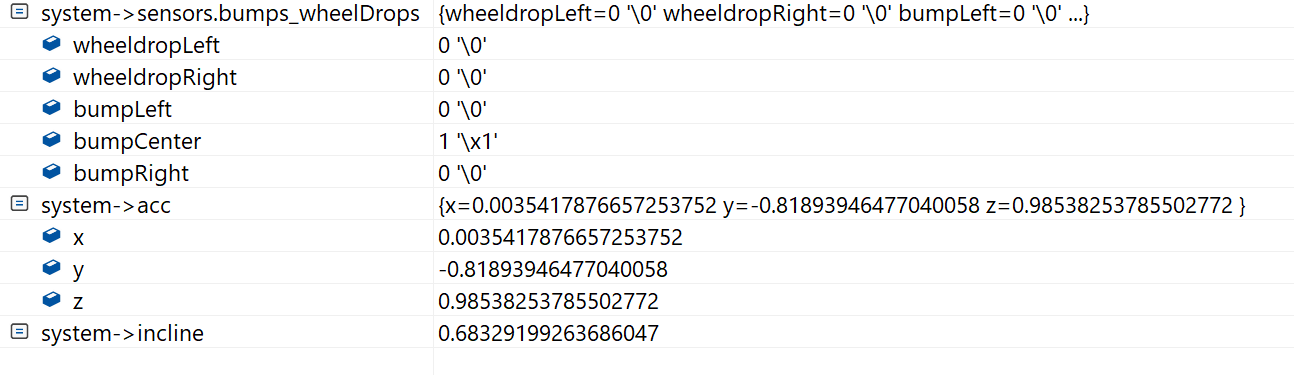
\includegraphics[width=0.8\textwidth]{Images/debug_incline}
    \caption{Debugging Simulation during Collision}
    \label{fig:debug_incline}
\end{figure}

In practice the state machine is synchronous because there is an update loop every 80ms. Our design fails to describe the behaviour of the system when two events happen in the same update. For example, there is no specification of the behaviour if an obstacle is detected in the centre and the right at the same time. Does the object location get set to be the centre or the right? This clearly indicates that our design introduces non-determinism. Non-determinism could have been implemented using a random number generator however in our implementation there is a precedence of transitions if multiple are triggered. Simply, the trigger that was declared earlier in the list of triggers will take precedence.
\paragraph{}
Furthermore, the design also does not indicate the behaviour if a transition is triggered at the same time as a trigger within the refinement of the current state. For example, if an incline is detected simultaneously with an obstacle detected, does the refinement enter the ``Ascending" state before the Kobuki reverses? Some implementations will have a precedence for transitions across hierarchies, however for our implementation, transitions will occur in the refinements before the higher level transitions. Perhaps, if only the higher level transition was allowed to occur then the unintentional hill-state transitions when colliding would be avoided.
\\
%could talk about making it concurrent? conurrent HFSMs are more powerful
\colorbox{yellow}{Pretty much have a whole page for this}